\documentclass[11pt,a4paper,oneside]{report}

% narrow margins, otherwise same layout as default
\AtBeginDocument{%
  \paperwidth\textwidth
  \advance\paperwidth48bp
  \oddsidemargin-48bp
  \paperheight\textheight
  \advance\paperheight48bp
  \advance\paperheight\headheight
  \advance\paperheight\headsep
  \advance\paperheight\footskip
  \topmargin=-48bp
  \pdfpagewidth=\paperwidth
  \pdfpageheight=\paperheight
}

\makeatletter
\long\def\@makecaption#1#2{%
  \vskip\abovecaptionskip
  \sbox\@tempboxa{\small \textbf{#1:} #2}%
  \ifdim \wd\@tempboxa >\hsize
    {\small \textbf{#1:} #2\par}
  \else
    \global \@minipagefalse
    \hb@xt@\hsize{\hfil\box\@tempboxa\hfil}%
  \fi
  \vskip\belowcaptionskip}
\makeatother

% fonts
\usepackage{tgpagella}
\let\slshape\itshape
\usepackage[TS1,T1]{fontenc}

\usepackage{array,textcomp,graphicx}
\setcounter{secnumdepth}{2}
\setcounter{tocdepth}{2}
\usepackage[%
  raiselinks=false,%
  colorlinks=true,%
  bookmarksnumbered=true,%
  bookmarksopen=true,%
  bookmarksopenlevel=1%
]{hyperref}
\pagestyle{headings}

\newcolumntype{P}[1]{%
  >{\raggedright\hspace{0pt}\arraybackslash}p{#1}}
\def\TL{\TeX~Live}
\def\fta{filetype association}
\def\FTA{Filetype association}
% if bold small caps available:
\def\mysc#1{{\rmfamily\textsc{#1}}}
% if bold small caps unavailable:
%\def\mysc#1{\textsc{\textmd{#1}}}
\def\GUI{\mysc{gui}}
\def\RUG{\mysc{rug}}
\def\UWP{\mysc{uwp}}

\def\TNC{TeXnicCenter}
\def\TS{TeXstudio}

\def\XeTeX{Xe\TeX}
\def\dbr{\discretionary{}{}{}}
\let\bsl\textbackslash
\def\bslb{\bsl\discretionary{}{}{}}
%\def\hkcu{HKEY\_\dbr CURRENT\_\dbr USER}
\def\hkcu{\textsc{hkcu}}
%\def\hklm{HKEY\_\dbr LOCAL\_\dbr MACHINE}
\def\hklm{\textsc{hklm}}
%\def\hkcr{HKEY\_\dbr CLASSES\_\dbr ROOT}
\def\hkcr{\textsc{hkcr}}
\newenvironment{ttdesc}{%
  \def\descriptionlabel##1{\hspace\labelsep\ttfamily\selectfont ##1}%
  \description}{\enddescription}
\hyphenation{head-ache work-space}

\title{TLaunch: a launcher for a \TL{} system}
\author{Siep Kroonenberg}
\begin{document}
\maketitle
\clearpage
\thispagestyle{empty}
\null\vfill
{\small\parindent=0pt
This manual is for tlaunch, the \TL{} Launcher, version 0.5.3.

Copyright \textcopyright{} 2017 Siep Kroonenberg.

Copying and distribution of this file, with or without modification,
are permitted in any medium without royalty provided the copyright
notice and this notice are preserved. This file is offered as-is,
without any warranty.\par}
\clearpage
\thispagestyle{empty}
% let physical pages match logical ones
\setcounter{page}{3}
\tableofcontents

\chapter{The launcher}
\label{chap:launcher}

\begin{figure}
  \centering
  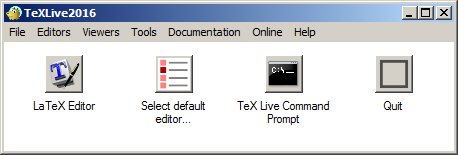
\includegraphics[width=.7\linewidth]{figures/tlaunch_window}
  \caption{A possible Launcher window}
  \label{fig:launcher}
\end{figure}

\section*{About this document}

This manual documents the \TL{} Launcher. The first chapter
describes the launcher in general, its facilities, its ini file and
its command-line parameters.

The second chapter describes the launcher-based installation at the
\RUG, or Rijksuniversiteit Groningen, as an example
launcher-based installation.

Since many \TeX{} developers spend as little time as they can help
in a Windows environment, I also added an appendix with Windows
background information.

\section{Introduction}
\label{sec:intro}

I designed the \TL{} launcher for the Windows \TL{} installation on
our university network, which contains \TL{} itself plus several
other \TeX-related applications.  The launcher provides a single
access point to all this software, and to related local and online
resources.

The launcher also takes care of configuration: at first run, \TL{}
is added to the searchpath, and relevant filetype associations are
set up.

This means that the launcher rather than the classic \TL{} installer
takes care of Windows-specific configuration. Which is a good
thing if the \TL{} directory tree is on a shared network drive, or
if a \TL{} installation has to be copied to many workstations.

Filetypes, menus and buttons and pre- and post configuration scripts
are defined in a standard Windows ini file. The format of this file
is described in section \ref{sec:config} of this chapter.  The
supplied ini file provides something more or less equivalent to a
classic Windows \TL{} installation.

\subsection{Localization}
\label{sec:localize}

Although at the moment the launcher lacks proper support for
localization, most of the user interface strings are defined in the
ini file and can be replaced with strings in other languages.

\section{Modes}
\label{sec:modes}

\subsection{Normal mode}
\label{sec:normal}

In a normal run, the launcher displays a window with a menu or a
series of buttons or both, see figure \ref{fig:launcher}. For
anything launched via these controls, \TL{} is prepended to its
process searchpath irrespective of the system- or user
searchpath; see Appendix \ref{sec:env} on Windows searchpath
handling.

\subsection{Initializing}
\label{sec:init}

On first run, tlaunch creates file associations and prepends \TL{} to
the user searchpath, see appendix~\ref{sec:env}. Such configuration
allows users to start up their \LaTeX{} editor by double-clicking a
\LaTeX{} file in their file manager, bypassing the launcher
altogether.

On first run, the launcher also creates a renamed copy of itself and
a renamed modified copy of the configuration file to a directory
inside the user's profile. This pair of copies serves as
\emph{forgetter}, see below. tlaunch registers this forgetter as an
uninstaller under Windows.

\subsection{Forgetting}
\label{sec:forget}

Since a network- or multi-user \TL{} installation can be uninstalled
by others, it is desirable that the configuration done on first run
can be reversed without the presence of the original \TL{}. The
forgetter takes care of this.

The launcher detects from its location whether it should run normally
or as forgetter.

It is also possible to undo configuration from within a normal run
if the ini file defines a button- or menu control for it.

\section{Using scripts}
\label{sec:scripts}

External scripts may run on demand, as the action associated with a
button or a menu control; see section \ref{sec:utscripts}. Scripts
may also run automatically, as supplemental initialization or
cleanup; see the \texttt{pre\_config}, \texttt{post\_config} and
\texttt{pre\_forget} variables in table \ref{tab:strings}. Examples:
\begin{itemize}
\item Forgetting a previous release of \TL{} before configuring the
  current one. This only makes sense for a centrally-managed \TeX{}
  installation, where it is known what \TeX{} installation came
  before.
  \item Giving \TeX works some spelling dictionaries
  \item Writing configuration data for non-\TL{} components
  \item Adjusting \XeTeX{} font configuration, see Section
    \ref{sec:xecache}
\end{itemize}

\section{The ini file}
\label{sec:config}

The ini file defines the menu items and buttons of the graphical
interface. These controls can start up \GUI{} programs or run
utility scripts, or run some predefined functions. The ini file also
defines filetype associations, and may specify scripts for doing
additional configuration and cleanup.

\subsection{Location}
\label{sec:loc}

In \TL, the binary is in the \TL{} binary directory,
\texttt{\emph{tlroot}/bin/win32}, and the ini file is in
\texttt{\emph{tlroot}/texmf-dist/web2c}. The installer may have
created a modified higher-priority copy in
\texttt{\emph{tlroot}/texmf-var/web2c}. A custom
\texttt{tlaunch.ini} in \texttt{\emph{tlroot}/texmf-config/web2c}
will override either. In this case, the filename database should be
updated.

Another option is to place both the binary and the ini file in the
root of the \TL{} installation.

\subsection{Encoding}
\label{sec:enc}

The launcher tries to guess the encoding used, and accepts
ASCII, UTF-8 and Windows' UTF-16, with or without BOM. If all else
fails, it tries ANSI with the system default code page.

\subsection{Syntax}
\label{sec:synt}

The ini file is a regular Windows ini file with sections,
definitions and comment lines.
\begin{itemize}
\item A section starts with a line containing the section name
  enclosed in square brackets `\texttt{[}' and `\texttt{]}'. It ends
  at the start of the next section or at the end of the file.
\item A definition line consists of a line
  \texttt{\emph{key}=\emph{value}}.
\item A comment line starts with `\texttt{;}'.
\end{itemize}

The ini file is processed in one go, which means that everything
must be defined before it is used. The ordering of the list below of
possible sections satisfies this requirement.

However, it is not necessary that everything that is referred to
actually exists; if a menu- or button control refers to a
non-existent file, the control is quietly left out, and if the
\texttt{COMMAND} of a filetype refers to a non-existent file then
neither the filetype registry entry nor any control for it will be
created.

The ini file can contain the following sections:

\subsection{The Strings section}
\label{sec:strings}

\begin{table}[tb]
  \centering
{\small
\extrarowheight3pt\sffamily\noindent
\begin{tabular}{|>{\ttfamily}llP{2in}|}
  \hline
  & DEFAULT & MEANING \\
  tlroot & predefined & root of the \TL{} installation \\
  version & predefined & release year \\
  tlperl & predefined & path of the built-in Perl binary \\
  tlwperl & predefined & same for the \GUI{} Perl binary \\
  java & predefined & Java binary, if found \\
  tlconfig & required & directory for the launcher's user data, see \emph{e.g.}
     sections \ref{sec:strings} and Appendix \ref{sec:known_configs} \\
  tlname & \texttt{TeX Live \%version\%} & used for \emph{e.g.}
      window title and uninstaller `DisplayName' \\
  customed\_progid & \texttt{TL.customed} & Filetype
      for external, user-selected editor, see section \ref{sec:fta} \\
  pre\_config & empty & optional program or script to be run before
      first-time initialization \\
  post\_config & empty & optional program or script to be run after
      first-time initialization \\
  pre\_forget & empty & optional program or script to be run before
      undoing initialization \\
  announce & empty & optional text to display \\[3pt]
  \hline
\end{tabular} \\[3pt]
Note. All process environment variables, \emph{e.g.}
\texttt{\%appdata\%}, are accessible while the
launcher parses the ini file. Variable names are case-insensitive.\par}

\caption{Strings with a special meaning in the ini file}
\label{tab:strings}
\end{table}

In this section arbitrary strings can be defined to be used later
during parsing. The names of the string variables are
case-insensitive, their values are not. Various strings have a
special meaning, see Table \ref{tab:strings}. Their values may be
predefined, \emph{i.e.} they are set by the launcher before
processing the ini file; they may be required, or they are allowed
to stay empty.

At a minimum, the \texttt{TLCONFIG} string should be defined in the
ini file. This is the directory for launcher user files such as the
forgetter. A few suggestions:
  \begin{itemize}
  \item \texttt{\%UserProfile\%\bsl.texlive\%version\%\bslb tlaunch},
    \emph{i.e.} under the common root of \texttt{\%TEXMFVAR\%} and
    \texttt{\%TEXMFCONFIG\%}
  \item \texttt{\%appdata\%\bslb tlaunch\bslb\%version\%}; see Appendix
      \ref{sec:known_configs}
  \item or maybe \texttt{\%localappdata\%\bslb tlaunch\bslb\%version\%} if
    \TL{} is installed on the local system
  \end{itemize}

\subsection{Sections for filetype associations (FTAs)}
\label{sec:fta}

In Windows, an extension is associated with a filetype and a
filetype is associated with a program. An extension can also have
alternate filetypes associated with it, which may show up if you
right-click a file and select `Open with\textellipsis'. More on
filetypes in appendix \ref{sec:wftas}.

A filetype section has as name the string `\texttt{FT:}' followed by
the filetype name. An example of a filetype section:

\begin{verbatim}
[FT:TL.TeXworks.edit.%VERSION%]
COMMAND="%tlroot%\bin\win32\TeXworks.exe"
;SHELL_CMD="%tlroot%\bin\win32\TeXworks.exe" "%1"
;ICON="%tlroot%\bin\win32\TeXworks.exe,0"
;NAME=TeXworks
EXTENSIONS=.tex .cls .sty
;PRIMARY=1
;PATH_PREFIX=0
\end{verbatim}

The commented lines are optional and represent default values.

\begin{ttdesc}
\item [COMMAND] is the command to start the program.
\item [SHELL\_CMD] is the command to open a file. The default is
  \texttt{COMMAND} with `\texttt{~"\%1"}' appended.
\item[ICON] is the icon to be used in GUI file managers. The default
  is \texttt{COMMAND} with `\texttt{,0}' appended, without a
  space. If there is no such icon then a fall-back icon will be
  used; see \emph{e.g.} the right-most icon in Figure
  \ref{fig:launcher}.
\item[NAME] is only used for \LaTeX{} editors, in the
  editor-selection window, see section \ref{sec:edsel}. If not
  specified, it will be derived from the program filename.
\item[EXTENSIONS] is the list of extensions that should have the
  filetype as primary or secondary association.
\item[PRIMARY] is default 1. If set to 0, then the program only
  shows up in the Open with... dialog. Mainly of interest for the
  bitmap2eps utility. See appendix \ref{sec:wftas} on primary and
  secondary filetypes.
\item[PATH\_PREFIX] is default 0. If set to 1, Windows will
  prepend \TL{} to the program's searchpath. The launcher will only
  do this if \texttt{COMMAND} is a bare or quoted filename, without
  options or parameters; see Appendix \ref{sec:appreg}.
\end{ttdesc}

\subsection{Sections for utility scripts}
\label{sec:utscripts}

A batchfile or command-line program can be declared in a
utility-script section. If a button or menu item invokes such a
script, standard output is intercepted and displayed in a dialog box
when the script has completed.  Standard error is also captured, but
shows up only in the log file \texttt{\%TEMP\%\bslb TeXLive\_\dbr
  Launcher.\dbr log}. A splash text is displayed while the script is
running. The default value for the splash text is `Working...'. An
example adapted from the \RUG{} installation:
\begin{verbatim}
[SC:TNC_config]
command=cscript "%TLROOT%\rugscripts\tnc_config.vbs" "%tlroot%"
;splash=Reconfiguring TeXnicCenter...
\end{verbatim}
In this example, the script takes just a moment, so there is no
point in defining a splash text.

\subsection{The built-in functions}
\label{sec:fun}

The following functions are available:
\begin{ttdesc}
\item [FU:quit] Terminate the launcher
\item [FU:clear] Undo all configuration and terminate
\item [FU:initialize] Undo all configuration, terminate and
  restart. This forces re-initialization.
\item [FU:editor\_select] See section \ref{sec:edsel}
\item [FU:default\_editor] See section \ref{sec:edsel}
\item [FU:about] An About box
\item [FU:uninst\_all] See section \ref{sec:lbased}
\item [FU:uninst] See section \ref{sec:lbased}
\end{ttdesc}

\subsection{Menus and buttons}
\label{sec:controls}

The visible interface of the launcher consists of an optional menu
with dropdown submenus and an optional row of buttons. There should be
at least one button or one submenu with one entry.

A submenu is defined in a section with name `\texttt{MN:}' followed
by the submenu name, and the row of buttons is defined in a section
named `\texttt{BUTTONS}'. A button- or a menu item has as key the
string to be displayed and as value one of the following:
\begin{itemize}
\item A filetype. This invokes its \texttt{COMMAND}.
\item A utility script. This also invokes its \texttt{COMMAND}.
\item `\texttt{SO:}' (Shell Open) followed by a document or
  \textsc{url}. The document or url will be opened in its default
  program.
\item A predefined function, see section \ref{sec:fun}.
\item An arbitrary command.
\end{itemize}
In a submenu section, a sole `\texttt{=}' will produce a separator
line. In the button section, it will do nothing.

{\sloppy
Example buttons- and submenu sections:
\begin{verbatim}
[MN:Tools]
Editor choice=FU:editor_select
TeX Live Command Prompt=%comspec% /T "TeX Live" /e:on
=
(Re)configure TeXnicCenter=SC:TNC_config

[MN:Documentation]
All TeX Live documentation by package=SO:%tlroot%\doc.html
TeX and LaTeX Q & A=SO:http://tex.stackexchange.com/

[BUTTONS]
LaTeX Editor=FU:default_editor
PostScript Viewer=FT:TL.PSView.view.%VERSION%
Quit=FU:quit
\end{verbatim}
\par}

\subsection{The General section}
\label{sec:gen}

This section is optional. Four keywords are allowed, of which the
first two correspond to \TL{} installer options:
\begin{ttdesc}
\item[Filetypes] Allowed values are
  \begin{itemize}
  \item \texttt{none}: do not set or change filetype associations
  \item \texttt{new}: create filetype associations only if they do
    not override existing ones; default
  \item \texttt{overwrite}: create filetype associations regardless
    of existing ones
  \end{itemize}
\item[searchpath] {\sloppy Allowed values are 0 (leave searchpath
    alone) and 1 (add \TL{} to the searchpath; default). See
    appendix \ref{sec:env}. In any case, when a program is started
    from the launcher it will have \TL{} prepended to its process
    searchpath.\par}
\item[remember] Allowed values are 0 (do nothing) and 1 (arrange
  that \TeX-related filetype associations are restored on
  login). This may be desirable in a Roaming Profiles setup, see
  sections \ref{sec:roam} and \ref{sec:noroam}.
\item[keeptemps] Allowed values are 0 (delete temporary files;
  default) and 1 (keep them). This is a debug option for running
  external scripts. In most cases however, the contents of the
  temporary files are copied to the log file \texttt{\%TEMP\%\bslb
    TeXLive\_\dbr Launcher.log} anyway.
\end{ttdesc}

An example general section:
\begin{verbatim}
[General]
FILETYPES=new
SEARCHPATH=1
KEEPTEMPS=0
\end{verbatim}
The above values are the defaults.

\section{Editor choice}
\label{sec:edsel}

\begin{figure}
  \centering
  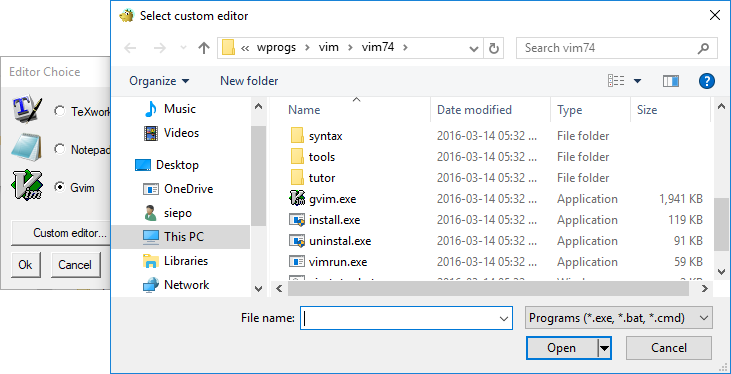
\includegraphics[width=.8\linewidth]{figures/custom_ed}
  \caption{Editor selection with a file browser for a custom editor}
  \label{fig:ed_sel}
\end{figure}
If a filetype has \texttt{.tex} among its supported extensions, the
launcher considers it an editor. On initialization, the first one
becomes the default, unless \texttt{PRIMARY} is set to 0 and there
is another candidate with \texttt{PRIMARY} 1. If in the
\texttt{General} section \texttt{FILETYPES} is set to \texttt{none}
or \texttt{new}, then an existing file association for \texttt{.tex}
files will not be overwritten.

The function \texttt{FU:default\_editor} invokes the default editor
if there is one. The function \texttt{FU:editor\_select} invokes a
dialog for selecting a default editor; the options are the ones
defined in the ini file, the current default and selecting one via a
file browser dialog, see figure \ref{fig:ed_sel}.

If the new editor is selected via the file browser, it will be
assigned to the filetype \texttt{TL.customed} and this filetype will
become the default for \texttt{.tex} files.  It is possible to
configure another filetype string in the ini file, \emph{e.g.} one
which includes the \texttt{\%VERSION\%} string.

Appendix \ref{sec:userchoice} explains why a \texttt{.tex} file
might still get opened in another editor.

\section{Launcher-based installations}
\label{sec:lbased}

It seems possible to do away with much of the Windows-specific code
of the current installer. To this end, I added install and uninstall
options to the launcher. Installation merely means creating a Start
menu entry for itself and to register itself as uninstaller.

In installation mode, it is assumed that the launcher and its ini
file are already in place as part of the regular \TL{}
installation.

The launcher can be invoked with the following command-line
parameters:

\begin{ttdesc}
\item[user\_inst] Install the launcher for a single user. This
  includes doing the first-time initialization as in a regular
  invocation.
\item[admin\_inst] Install the launcher for all users
\item[uninst] Undo installation but leave the \TL{}
  directory tree alone. Also runs the forgetter for the current
  user silently, if it exists.
\item[uninst\_all] Undo installation and remove the \TL{} directory
  tree. Also runs the forgetter for the current user silently, if it
  exists. This is the only option of these four which touches the
  \TL{} installation itself.
\item[remember] Recreate filetype associations, see sections
  \ref{sec:roam} and \ref{sec:noroam}.
\item[silent] Do not ask for confirmation and do not pop up
  messages. Output is still written to the log file, at
  \texttt{\%TEMP\%\bslb TeXLive\_\dbr Launcher.\dbr log}.
\end{ttdesc}
The \texttt{user\_inst\_silent} and \texttt{admin\_inst\_silent} are
also still available.

The non-silent uninstall options both ask which of the two uninstall
options is desired. the only difference between them is which button
is the default.

The new launcher mode option of the 2017 \TL{} installer invokes the
launcher with one of the silent installer options.

Within the launcher, there are functions \texttt{FU:uninst\_all} and
\texttt{FU:uninst} which can be assigned to a menu- or button
control. If necessary, the launcher will pop up a \textsc{uac}
prompt and restart in elevated mode.

The \TL{} installer may create a higher-priority
\texttt{tlaunch.ini} if for either the path setting option or the
file associations option a non-default value was selected. This will
happen even if launcher mode was not selected.

\subsection{The tlaunchmode script}
\label{sec:tlaunchmode}

The included Perl script tlaunchmode can convert a local \TL{}
installation between classic and launcher-based. Run with a
parameter `on', the script turns launcher mode on; with `off' it
reverts the installation to classic, and anything else prints a
brief help message.  It is already part of \TL.

It aborts if admin permissions are required but missing.

\subsection{\TeX{} Live Manager}

Nothing special has been done for the \TL{} Manager. It can be
assigned to a menu- or button control, although this makes little
sense for a centrally managed network installation. If necessary it
will automatically pop up a \textsc{uac} prompt.

\chapter[The launcher at the RUG]{The launcher at the
  Rijksuniversiteit Groningen}
\label{chap:rug}

\begin{figure}[tb]
  \centering
  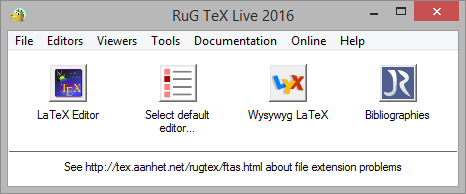
\includegraphics[width=.7\linewidth]{figures/tlaunch_rug}
  \caption{The launcher at the Rijksuniversiteit Groningen}
  \label{fig:launcher_rug}
\end{figure}

This chapter deals with the launcher-based \TL{} installation at the
\RUG{} (Rijksuniversiteit Groningen) and the environment in which it
operates.

Our \TL{} installation resides on the network.  The \TL{} Launcher
is available via a centrally managed start menu. From any Windows
workstation connected to the network, one can click the launcher
shortcut in this menu and start using \TeX{}.

The files in the \texttt{tlrug.zip} zipfile are tidied up versions
of those of the \RUG{} installation; they omit some ugly workarounds
for specific local problems and also benefit from hindsight.

\section{Historical}

An earlier solution for \TL{} was implemented with a patchwork of
scripts in various languages. An initialization script created
filetype associations, Start Menu shortcuts and modified the
searchpath. It made use of the built-in Perl and its \TL{} modules.

When between 2013 to 2014 the university transitioned to centrally
managed desktops, using the RES workspace management
system\footnote{Real Enterprise Solutions,
  \texttt{https://res.com/}}, I created the launcher.  Because
previously users might run the initializer / installer when they
really want to run the already initialized / installed \TL, I opted
this time for a launcher that configures itself automatically,
without requiring a separate initialization step.

For speed of development, a first version was written in the
AutoIT\footnote{\texttt{https://\dbr www.\dbr autoitscript.\dbr
    com/}} scripting language. AutoIT has good access to Windows'
internals, and comes with a utility which packages a script with a
AutoIT runtime into a self-contained executable. The AutoIT versions
did not use an ini file; everything was coded into the script
itself.

For the 2015 \TL{} release, I finally had a usable C version, in
which all configuration was read from an ini file.

\section{RES desktops}
\label{sec:res}

The RES system synthesizes a desktop or workspace for the user on
logon. Personal settings are selectively captured, stored in a
database and restored on re-logon; the settings part of RES can be
considered an alternative implementation of the roaming profiles
described in Appendix \ref{sec:roam}.

This desktop is also available remotely, which works reasonably well
most of the time.

For \TL, I submit a wish list of settings to be captured to the
workspace management people, and they enter everything into the RES
system. Unfortunately, the RES system has its quirks, and what I
expect to happen is not always what actually does happen. Some of
these problems are mentioned later on.

\section{Components of the \RUG{} \TeX{} installation}
\label{sec:comps}

Various third-party programs are incorporated into our \TL{}
installation. Below are some details.

Most \TeX-related software does not have deep hooks into the
system. Even if applications require elevated permissions to
install, usuallly they can simply be copied to another location and
work fine from there. This is the case with \emph{e.g.}  \TL{}
itself and with \TS.

The add-ons are:
\begin{itemize}
\item Additional editors: \TNC{} and \TS{}
\item The pdf viewer SumatraPDF
\item The Java-based bibliography manager JabRef
\item The epspdf \GUI{} with bundled single-file Tcl/Tk runtime
\item The pseudo-wysywyg LyX \LaTeX{} editor
\end{itemize}
There are also controls for:
\begin{itemize}
\item browsing the \TL{} installation
\item a command-prompt with \TL{} as the first directory on the
  searchpath
\item some manuals from the \TL{} installation
\item links to \TeX-related websites
\end{itemize}
Such menu items are simply created by single lines in the
ini file.

There are no controls for the \TL{} manager or for uninstalling.

Figure \ref{fig:launcher_rug} shows buttons for some of the
additional software. Along the bottom of the window is an
announcement text, which is an optional string item in the ini
file. The Help menu item opens a help text in the configured default
text editor -- probably Notepad.

\section{Directory organization}
\label{sec:rugdirs}

There is a directory under the \TL{} root containing all the
extras. There is another subdirectory for the various scripts. All
paths in both the ini file and the scripts are relative to the root
of the installation.

I placed both the binary and the ini file in the root of the
installation, but did not place anything into existing \TL{}
subdirectories.

\section{Fixes for add-ons}
\label{sec:fixes}

Some of the add-ons needed a bit more work than just copying the
installed program directory to its place under the \TL{} root:

\subsection{\TNC}
\label{sec:tnc}
The original university installation was based on MikTeX, with
\TNC{} as editor. In 2008 I replaced MikTeX with \TL, and \TNC{}
with the more up to date \TS{} editor. Since I did not want to force
anyone to switch editors, I also kept \TNC{} around.

While \TNC{} can autoconfigure itself nicely for MikTeX, it asks
\TL{} users a series of questions about what is where. Since many
users do not know their way around outside their home directory, I
wrote a vbscript which emulates the MiKTeX autoconfiguration for
\TL{} and spares the user awkward questions.

\subsection{\TS}
\label{sec:ts}

\TS{} autoconfigures itself fine, but there were still two problems:
\begin{enumerate}
\item By default, it checks whether there is a more recent version,
  while users are not in a position to do an update themselves.
\item With our current desktop management software, programs do not
  get the user searchpath appended to their process searchpath.
\end{enumerate}
The first problem is solved during first-time initialization of the
launcher. If there is no \TS{} configuration file, then one is
created with just the setting not to check for updates. If there is
one, the update check option is edited to be off. Either way, there
is no impact on other settings.

A possible solution for the second problem is described in Appendix
\ref{sec:appreg}, but I opted instead to start \TS{} via a small
wrapper program.

Note that the \TL{} runscript wrapper does already take care of the
searchpath for TeXworks, Dviout and PSV[iew].

\subsection{SumatraPDF}
\label{sec:sumatra}

In the absence of any registry settings, SumatraPDF assumes that it
is a portable setup, and tries to write user configuration to its
own directory. Following advice from its developers, I created a
registry setting to tell SumatraPDF otherwise, and let it write
its configuration data to the user's profile.

Checks for updates are disabled in a similar way as for \TS.

\subsection{LyX}
\label{sec:lyx}

On first start, LyX can take several minutes to take stock of its
environment and figure out what it can use. During this time, it is not
even clear that anything is happening.

To prevent this delay, the post-config script copies a pre-generated
configuration directory to the user's profile.

In the LyX installation itself, in the file
\texttt{\emph{lyxroot}\bslb Resources\bslb lyxrc.dist}, the setting
\texttt{\bsl path\_prefix} has been rephrased to only contain paths
relative to \texttt{\$LyXDir}, which is the root of the LyX
installation.

\section{Moving the \XeTeX{} font cache}
\label{sec:xecache}

The default location of the \XeTeX{} font cache in \TL{} is
\texttt{\$TEXMFYSVAR/\dbr fonts/\dbr cache}, \emph{i.e.}
\texttt{\emph{tlroot}/\dbr texmf-var/\dbr fonts/\dbr cache}. In a
multi-user or network install, this location is not
user-writable. Since this may be a problem,\footnote{\emph{E.g.} if
  the set of Windows fonts changes, \XeTeX{} will try to update the
  font cache but will not be able to save the updated cache.} a line
\begin{verbatim}
FC_CACHEDIR = $TEXMFVAR/fonts/cache
\end{verbatim}
in the file \texttt{\emph{tlroot}/\dbr texmf.cnf} will move the
cache to a user-writable location. The \texttt{tlaunchmode} script,
see section \ref{sec:tlaunchmode}, will take care of this
automatically.

Since I generate the \TL{} installation on a Linux system, the
configured \TL{} font paths in \texttt{\$TEXMFSYSVAR/\dbr fonts/\dbr
  conf/\dbr fonts.conf} do not match the target installation. Of
course this generated file can be hand-edited, but I preferred to
leave this file alone and move the font cache configuration files
also to a user-writable location with another line:
\begin{verbatim}
FONTCONFIG_PATH = $TEXMFVAR/fonts/conf
\end{verbatim}
in \texttt{\emph{tlroot}/texmf.cnf}. A per-user font configuration
is then created by a line
\begin{verbatim}
"%TLROOT%\tlpkg\tlperl\bin\perl.exe"
  "%TLROOT%\tlpkg\tlpostcode\xetex.pl"
  install "%TLROOT%" skip_gen 2>NUL
\end{verbatim}
(one line) in a post-config script, see section \ref{sec:scripts}.

The last parameter, \emph{viz.}  \texttt{skip\_gen}, suppresses
actual cache generation, since that might take quite some time and
only benefit \XeTeX{} users. Any non-null value would have had the
same effect.

\appendix

\chapter{Windows issues}

\section{User and system}
\label{sec:usersys}

Microsoft has wised up a lot security-wise. When Windows XP
appeared, the line of Windows 9\emph{x} windowses made place for
slightly crippled versions of the NT-based professional
editions. Even for Home editions there is now a separation between
per-user and system-wide settings and files. Since Windows Vista,
this separation is much more strictly enforced, and even
administrators have to take an extra step, such as clicking yes to a
UAC\footnote{User Account Control} prompt, before they can do
anything deemed risky.

\section{Roaming}
\label{sec:roam}

On a Windows domain network, it can be arranged that users have more
or less the same desktop, whatever computer within the network they
happen to be working on. This is accomplished by either `folder
redirection', \emph{i.e.} defining network locations for certain
dedicated directories (see `Known Folders' in Appendix
\ref{sec:known}), or by copying user data back and forth between
workstation and network on logoff and logon. There may also be a
dedicated network share for user documents which is accessible from
any computer, and which may do double duty as home to redirected
folders.

\section{Windows configuration}
\label{sec:wconfig}

Some Windows configuration can only be stored in the registry, in
particular file associations, see section \ref{sec:wftas} below, and
environment variables, including the searchpath.

Other configuration can be stored either in the registry or in
configuration files, at the discretion of the developer.

\subsection{Registry locations}
\label{sec:hives}

We have to deal with three locations or hives within the registry:
\begin{itemize}
\item \texttt{HKEY\_\dbr
    CURRENT\_\dbr USER}, or \hkcu{} in short, for user-specific settings
\item \texttt{HKEY\_\dbr
    LOCAL\_\dbr MACHINE}, or \hklm{} in short, for system-level settings
\item A third hive, \texttt{HKEY\_\dbr CLASSES\_\dbr ROOT}, or
  \hkcr, will be described in the next subsection.
\end{itemize}

\subsection{Filetype associations}
\label{sec:wftas}

The basic idea is that an extension has a default filetype or
ProgID, and this filetype in its turn can define commands such as
open, edit, view or print.  For example, the extension \texttt{.jar}
has as its filetype or ProgID \texttt{jarfile}, and for the ProgID
\texttt{jarfile} the open command is defined as \emph{e.g.}\par
{\footnotesize
\begin{verbatim}
"C:\Program Files (x86)\Java\jre1.8.0_45\bin\javaw.exe" -jar "%1" %*
\end{verbatim}
}\normalsize
Extensions can also have secondary file associations. These are
the ones showing up when right-clicking a file and selecting `Open
with\textellipsis'.

Filetype associations exist in per-user and system-wide flavors:

{\sloppy
\begin{itemize}
\item User-specific filetype associations are stored in
  \hkcu\texttt{\bslb Software\bslb Classes}
\item System-level filetype associations are stored in
  \hklm\texttt{\bslb Software\bslb Classes}
\item The effective filetype associations are stored in
  \texttt{HKEY\_\dbr CLASSES\_\dbr ROOT} or \hkcr, which is a
  runtime merge of the above two branches. Settings in \hkcu{}
  override corresponding settings in \hklm.
\end{itemize}}

{\sloppy For example, the link from \texttt{.jar} to
  \texttt{jarfile} is can be read from the \hkcr\texttt{\bslb.jar}
  key and the link from \texttt{jarfile} to actual commands from the
  \hkcr \texttt{\bslb jarfile} key.\footnote{In some situations,
    reading from \hkcr{} proved not entirely reliable. Therefore, \TL{}
    always explicitly checks first \hkcu{} and if necessary
    \hklm.}\par}

Secondary filetype associations can be stored in a subkey of the
extension subkey, either the \texttt{OpenWithList} (obsolete) or
the \texttt{OpenWithProgIds} subkey.

\subsection{Non-roaming filetype associations}
\label{sec:noroam}

{\sloppy
Unfortunately, these filetype associations do not roam.  With the
RES desktop management system at our university, this is no longer a
problem for us. For other setups, the launcher contains a workaround
which is activated by the \texttt{remember} ini file setting, see
section \ref{sec:gen}.\par}

When this is set to 1, the launcher will during first-time
initialization place a shortcut to the forgetter in the Start / All
Programs / Startup menu, with a `remember' parameter added. This
will cause the forgetter to run automatically at logon with a
remember parameter. With this parameter, it will just silently
recreate the filetype associations and then terminate.

\subsection{UserChoice}
\label{sec:userchoice}

{\sloppy
Apart from the registry settings under the two \texttt{\bslb
  Software\bslb Classes} keys, choices made by the user in the `Open
with\textellipsis' dialog are stored under subkeys of \hkcu
\texttt{\bslb Software\bslb Microsoft\bslb Windows\bslb
  CurrentVersion\bslb Explorer\bslb FileExts\bslb \emph{.ext}}, the
exact subkey(s) depending on the Windows version. Such entries
should have priority over the ones described above, and do roam.\par}

Windows 8 and later may pop up a dialog asking with what program to
open a file even if there is already an answer in a
\texttt{Software\bslb Classes} key. The answer will be a preference
stored under the \texttt{FileExts} key mentioned above. This should
alleviate the problem of non-roaming filetype associations.

The launcher will not touch these registry entries.

\subsection{Application registration}
\label{sec:appreg}

An application which is registered may have a better chance to be listed
as an alternative in the `Open with...' dialog.

{\sloppy The currently recommended way to register an application is
  under the \texttt{SOFTWARE\bsl Microsoft\bslb Windows\bslb
    CurrentVersion\bslb App Paths\bslb \emph{basename}} key
  (\texttt{basename} including \texttt{.exe} file extension). The
  default entry of such a key is the full path of the
  file. Therefore, only one file with a given basename can have such
  a registration entry.\par}

The other entry of interest under this key is `Path', which is a
searchpath fragment that should be prepended to the regular
searchpath, just for this program. This prefixing happens if the
program is opened by Windows Explorer. The path prefix is ignored
if the program is started from the command-line or from the
launcher.

For filetypes defined in the launcher ini file, the launcher creates
an application registration key for the associated program, but only
if the \texttt{COMMAND} field is just a filename or -path, with or
without quotes.

{\sloppy
Applications can also be registered under \hkcr \texttt{\bslb
  Applications\bslb \emph{basename}}, but here is no option to set a
searchpath prefix. Microsoft considers this location obsolete.\par}

\subsection{The searchpath and other environment variables}
\label{sec:env}

Environment variables are also stored in the registry: per-user
variables in \hkcu\texttt{\bslb software\bslb environment}, system
environment variables in \hklm\texttt{\bslb System\bslb
  CurrentControlSet\bslb Control\bslb Session Manager\bslb
  Environment}.

For the searchpath, the effective searchpath consists of the system
\texttt{\%Path\%} variable, with the user \texttt{\%Path\%} variable
\emph{appended} if it exists, with an intervening `;' of
course. Therefore, \emph{directories on the system searchpath have
  priority over the user searchpath}.

Other environment variables from these registry locations behave as
expected: the user version has priority if both exist. Note that the
names of environment variables are case-insensitive.

{\sloppy
Various pieces of system information, such as \texttt{COMPUTERNAME}
and \texttt{CommonProgramFiles}, are not explicitly stored as
environment variables, but are nevertheless available as such.\par}

\section{ Windows Known Folders}
\label{sec:known}

Windows has an elaborate and ever expanding system of `Known
Folders': \emph{e.g.}  Program Files, ProgramData, User Profile
(HOME directory), Start Menu, Desktop, Documents, Downloads,
History, SendTo, Templates, Administrative Tools, Pictures, Music,
Videos, Account Pictures, Cookies, Favorites, and dozens more, many
of them both in a system- and a user version.

Sometimes a known folder is not a real folder but a virtual one, and
for some known folders, 64-bits applications and 32-bits
applications view things differently.

There are APIs which associate known folder identifiers to actual
directory paths.

With Windows Vista a new API has been introduced, and the old one
declared obsolete. One change for the better: the directory
name `Documents and Settings' has been replaced with simply `Users'.

This API also gives access to other properties, such as the
localized names shown in Windows Explorer, such as `Programme'
instead of `Program Files', or `Gebruikers' instead of `Users'.

Microsoft recommends to avoid hard-coded paths, and to place
everything under known folders instead. One benefit is at least that
files in known folders have a better chance of surviving system
upgrades.

\subsection{Programs}
\label{sec:knownprogs}

The directory reserved for programs is normally \texttt{c:\bslb
  Program Files}. On 64-bit systems, this directory is reserved for
64-bits programs, and \texttt{c:\bslb Program Files (x86)} for
32-bits programs. Directories under one of the Program Files folders
are automatically write-protected.

\subsection{Configuration- and data files}
\label{sec:known_configs}

There are also preferred locations for per-user- and system-wide
program data. For Windows Vista and later these are:
\begin{itemize}
\item {\sloppy For user-specific settings, typical locations are
  \texttt{\%appdata\%}, which is usually
  \texttt{\%userprofile\%\bslb \%appdata\%\bslb roaming}, and
  \texttt{\%localappdata\%}, which is usually
  \texttt{\%userprofile\%\bslb \%appdata\%\bslb local}. For a
  networked workstation, \texttt{\%appdata\%} may be relocated or
  backed up to a location on the network, and be available to the
  user on any workstation.\par}
\item {\sloppy For system-wide settings there is \texttt{\%ProgramData\%},
  usually \texttt{C:\bsl ProgramData}.\par}
\end{itemize}
On Windows Vista and later, these directories normally do \emph{not}
have spaces in their path. They are by default also hidden.

\subsection{\TL{} choices}
\label{sec:known_tl}

It is clear that \TL{} does not try very hard to conform to all
Microsoft's recommendations, and I do not think that it should. A
couple of obvious advantages of the existing default path
\texttt{C:\bslb texlive\bslb \emph{yyyy}}\footnote{Regular users can
  create directories in the root directory of the C:-drive, even
  though they cannot create regular files there.} are the absence of
spaces, and the locale-independence of the path seen in Windows
Explorer.

In this default location, \TL{} will not be write-protected
automatically.  For a system-wide installation, the \TL{} installer
itself will take care of this.

{\sloppy
As to user files, it should be ok to put \texttt{\$TEXMFCONFIG},
\texttt{\$TEXMFVAR} and tlaunch's \texttt{\%TLCONFIG\%} under
\texttt{\%appdata\%} or \texttt{\%localappdata\%}. For the first
two, this could also be done after the fact with a couple of lines
in \texttt{\emph{tlroot}/texmf.cnf}, \emph{e.g.}:
\begin{verbatim}
TEXMFVAR = $APPDATA/texlive2017/texmf-var
TEXMFCONFIG = $APPDATA/texlive2017/texmf-config
\end{verbatim}
There they will be hidden, but most users will never interact
directly with files in these directories anyway.\par}

\end{document}
